\documentclass[25pt, a0paper, portrait, margin=0mm, innermargin=15mm,blockverticalspace=15mm, colspace=15mm, subcolspace=8mm]{tikzposter}

\usepackage{fontspec}
\usepackage{multirow}
\usepackage{url}
\usepackage{alltt}
\usepackage{color}
%\usepackage[table]{xcolor}

\defaultfontfeatures{PunctuationSpace=3,Scale=MatchLowercase,Mapping=tex-text}

\setromanfont[Scale=1.1]{Liberation Serif}
\setmonofont{DejaVu Sans Mono}

\definecolor{darkgreen}{RGB}{0,127,0}

\settitle{ \centering \vbox{
%\@titlegraphic \\[\TP@titlegraphictotitledistance] \centering
\color{titlefgcolor} {\bfseries \Huge \sc \@title \par}
\vspace*{1em}
{\LARGE \@author \par} \vspace*{1em} {\Large \@institute}
}}

\makeatletter
\def\title#1{\gdef\@title{\scalebox{\TP@titletextscale}{%
\begin{minipage}[t]{1.0\linewidth}
\centering
#1
\par
\vspace{0.5em}
\end{minipage}%
}}}
\makeatother

\title{Unsupervised training of maximum-entropy models 
 for lexical selection in rule-based machine translation}
 \institute{$^\star$UiT Norgga árktalaš universitehta, $^\dagger$Universitat d'Alacant} % See Section 4.1
\author{Francis M. Tyers,$^\star$ Felipe Sánchez-Martínez,$^\dagger$ Mikel L. Forcada$^\dagger$} 
%\titlegraphic{
%
\includegraphics[width=0.04\textwidth]{LogoSamisk.png} \hspace{20pt}
%
\includegraphics[width=0.15\textwidth]{logodlsioficialcolor.eps} 
%}
%\usetheme{Basic} % See Section 5
\begin{document}


\maketitle % See Section 4.1
\begin{columns} % See Section 4.4

\column{0.50} % See Section 4.4

\block[titleinnersep=10em]{Lexical selection}{

  \begin{itemize}
    \item Lexical selection is:
    \begin{itemize}
    \item Choosing the most adequate 
translation for a word from a 
set of possibilities.
    \end{itemize}
    \item Why unsupervised ? 
    \begin{itemize}
      \item For many language pairs, parallel corpora are not available
    \end{itemize}
    \item Why maximum entropy ? 
    \begin{itemize}
      \item Allows linguists to define features for which weights are learnt.
    \end{itemize}
  \end{itemize}

}

  \block[titleinnersep=10em]{Apertium (\url{www.apertium.org})}{
    \begin{center}
      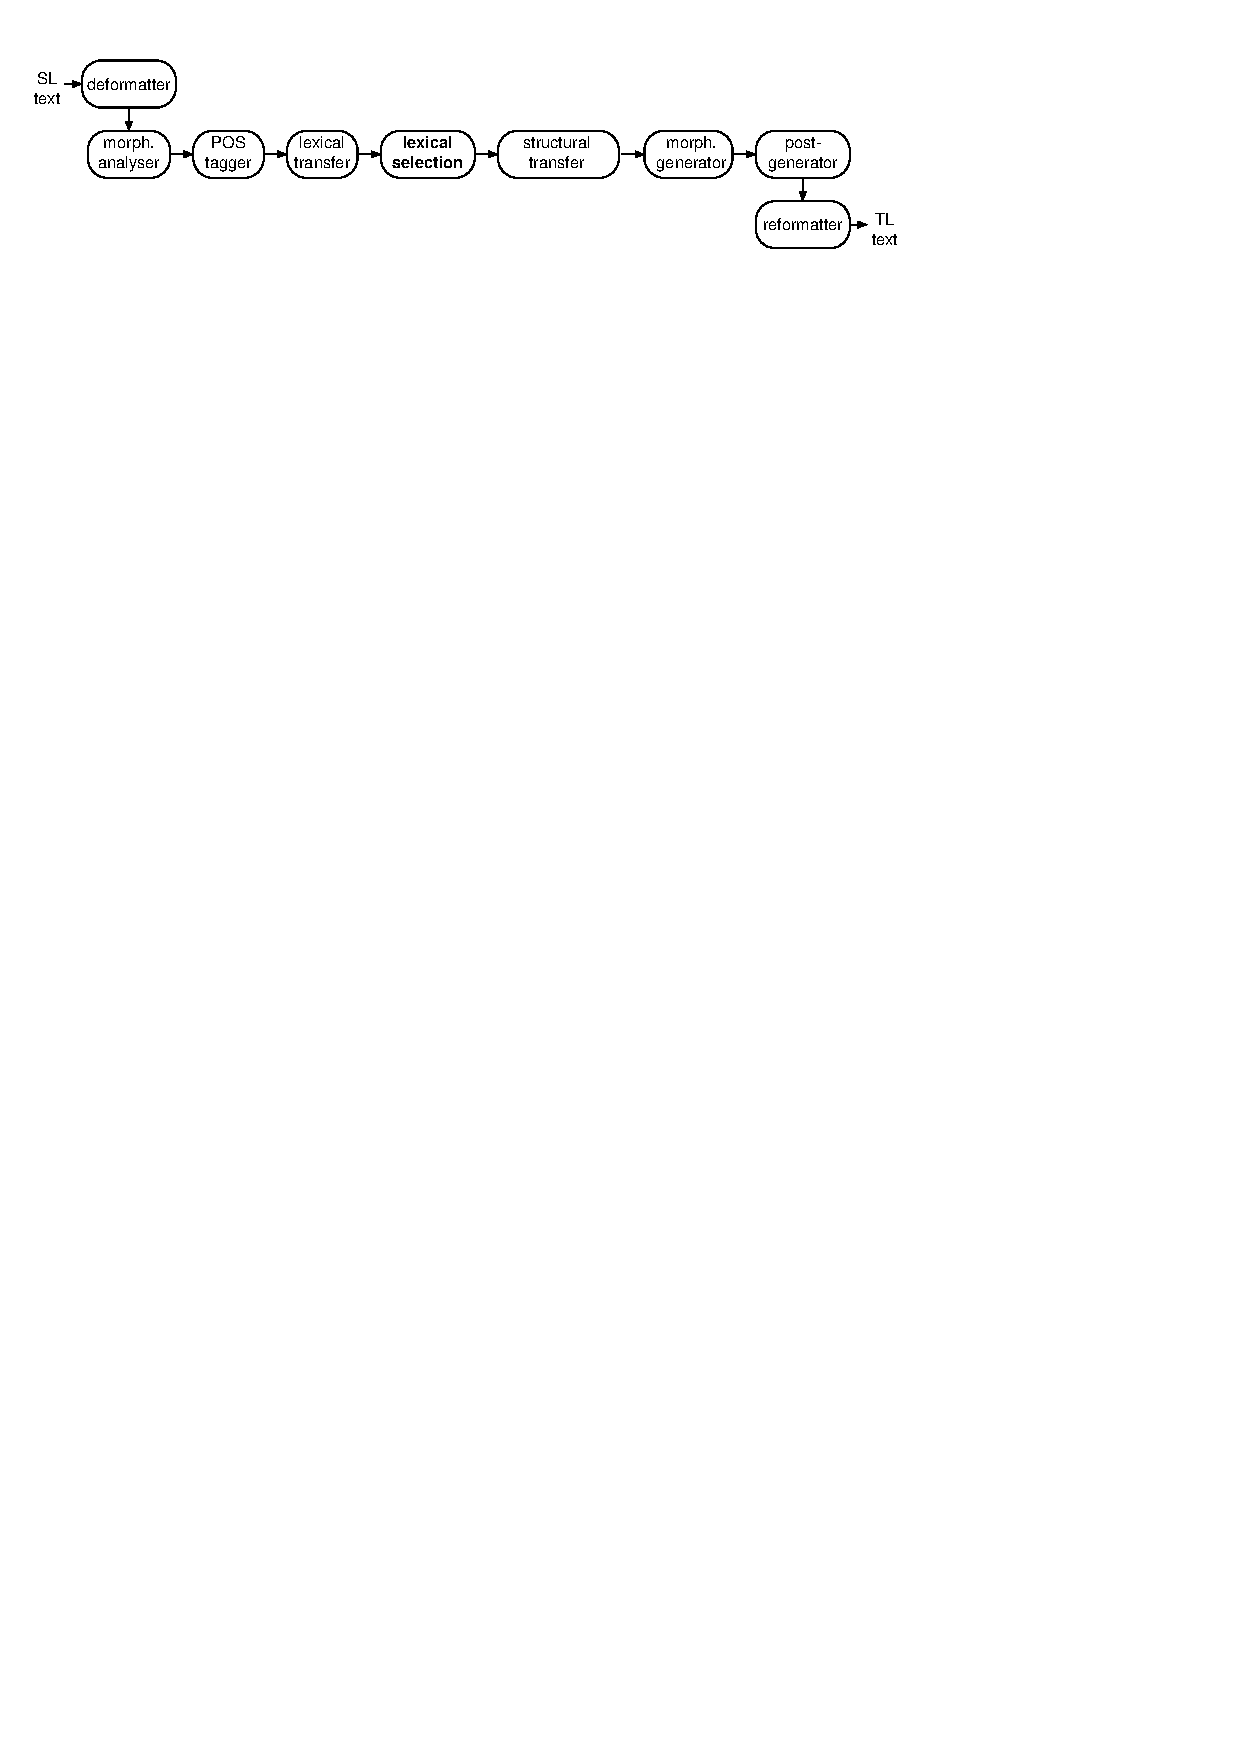
\includegraphics[width=0.45\textwidth]{architecture-lexsel.pdf}
    \end{center}
    \begin{itemize}
      \item Free/open-source RBMT platform
      \item Around 40 released language pairs
    \end{itemize}
  }
% -- weights should go on operations
%  <rule weight="0.906306">
%    <match lemma="ondare" tags="n"><select lemma="acervo" tags="n.*"/></match>
%    <match lemma="historiko" tags="adj.*"/>
%  </rule>
%  <rule weight="1.08987">
%    <match lemma="ondare" tags="n"><select lemma="patrimonio" tags="n.*"/></match>
%    <match lemma="historiko" tags="adj.*"/>
%  </rule>
%

  \block[titleinnersep=10em]{Training schema}{

%\begin{displaymath}
%    \label{eq:steps}
%    S \to \mbox{\framebox{\parbox{4.0cm}{\textit{pre-lexsel}}}} \to (\{g_i\}_{i=1}^{i=|G|},S) \to \mbox{\framebox{\parbox{3.5cm}{\textit{\textbf{lexsel}}}}} \to (g^\star,S) \to \mbox{\framebox{\parbox{4.0cm}{\textit{post- lexsel}}}} \to \tau(g^\star,S)
%  \end{displaymath}


  \begin{center}
    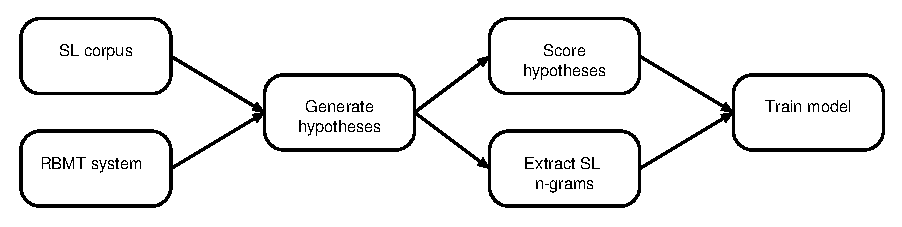
\includegraphics[width=0.45\textwidth]{schema.eps}
  \end{center}
  }

\column{0.5}
 

\block[titleinnersep=10em]{Training}{ % See Section 4.2

Translate SL sentences to TL using existing MT system and score the translations.

\useinnerblockstyle{Table}
\begin{center}
\begin{tabular}{|c|l|r|}
     \hline
        & \textbf{Sentence} & $p(g_i|S)$ \\
     \hline % Los pescados grandes peque\~{n}o come
      \(S_1\) & \emph{Arrain handiak txikia jaten du}  &  \\
                         $\tau(g_{1},S_1)$ & El pez grande se come el peque\~{n}o &  0.831 \\
                         $\tau(g_{2},S_1)$ & El pescado grande se come el peque\~{n}o & 0.169 \\
     \hline % El padre el pescado nos ha preparado para cenar
      \(S_2\) & \emph{Aitak arraina prestatu digu afaltzeko} &  \\
                         $\tau(g_{1},S_2)$ & Padre nos ha preparado pescado para cenar & 0.980 \\
                         $\tau(g_{2},S_2)$ & Padre nos ha preparado pez para cenar & 0.020 \\
     \hline % Aqu\'{\i} el pescado muy es dulce
     $S_3$  & \emph{Hemen arraina oso goxoa da}  & \\
                         $\tau(g_{1},S_3)$ & Aqu\'{\i} el pescado es muy rico & 0.980 \\
                         $\tau(g_{2},S_3)$ & Aqu\'{\i} el pez es muy rico & 0.020 \\
     \hline % Un pescado grande del mar es
     \(S_4\) & \emph{Itsasoko arrain handi bat da} & \\
                         $\tau(g_{1},S_4)$ & Es un pez grande del mar & 0.596 \\
                         $\tau(g_{2},S_4)$ & Es un pescado grande del mar & 0.404 \\
     \hline % El pescado grande por esos serv\'{\i}an para alimentar
     $S_5$ &  \emph{Arrain handiak horiez baliatzen ziren elikatzeko} &  \\
                         $\tau(g_{1},S_5)$ & Los peces grandes se nutr\'{\i}an de esos & 0.876 \\
                         $\tau(g_{2},S_5)$ & Los pescados grandes se nutr\'{\i}an de esos & 0.124 \\
     \hline
   
   \end{tabular}
\end{center}
}

\block[titleinnersep=10em]{Model}{

Extract $n$-gram contexts and train MaxEnt model.

\begin{center}
\begin{tabular}{|l|r|l|r|}
\hline
$h^s(t,c)$ & $\lambda$ & $h^s(t,c)$ & $\lambda$ \\
\hline
arrain:pez & 1.1356 & arrain:pescado & 0.90723 \\
aita arrain:pez & 0.167523 & aita arrain:pescado & 1.28196 \\
arrain:pez handi & 1.37525 & arrain:pescado handi & 0.49622 \\ 
arrain:pez oso & 0.167523 & arrain:pescado oso & 1.28196  \\ 
arrain:pez prestatu & 0.167523 & arrain:pescado prestatu & 1.28196  \\
hemen arrain:pez & 0.167523 & hemen arrain:pescado & 1.28196 \\ 
itsaso arrain:pez & 0.8466  & itsaso arrain:pescado & 1.40647  \\

\hline
\end{tabular}
\end{center}
%1.1356   arrain:pez \\
%0.90723  arrain:pescado \\
%1.28196  aita\_arrain:pescado \\
%0.167523 aita\_arrain:pez \\
%0.49622  arrain:pescado\_handi \\
%1.37525  arrain:pez\_handi\\
%1.28196  arrain:pescado\_oso \\
%0.167523 arrain:pez\_oso \\

%1.28196  arrain:pescado\_prestatu \\
%0.167523 arrain:pez\_prestatu \\
%1.28196  hemen\_arrain:pescado \\
%0.167523 hemen\_arrain:pez \\
%1.40647  itsaso\_arrain:pescado \\
%0.8466   itsaso\_arrain:pez \\
%\end{alltt}
}



\end{columns}

\block[titleinnersep=10em]{« Gaur arraina prestatuko dut. »}{

Compile features into finite-state transducer. 

    \begin{center}
      \includegraphics[width=0.70\textwidth]{transducer2.eps}
    \end{center}
\vspace{-20pt}
    arrain:pez = 1.303123 //
    arrain:pescado = 2.18919

The translation with the highest probability is one with the highest sum of the weights.

\begin{equation}
  \underset{t \in T_s(s)}{\arg\max} ~ p_s(t|c) = \underset{t \in T_s(s)}{\arg\max} \sum_{k=1}^{n_F} \lambda_k^s h_k^s(t, c)
\label{eq:max-ent-max}
\end{equation}

  }

\begin{columns}

%\block[titleinnersep=10em]{Training}{
%
%\begin{alltt}
%0 \$ 0.830 \# arrain:0 arrain\_handi:0 \# arrain:1 arrain\_handi:1  \# \\
%1 \$ 0.134 \# arrain:0 arrain\_handi:0 \# arrain:1 arrain\_handi:1  \# \\
%1 \$ 0.034 \# arrain:0 arrain\_handi:0 \# arrain:1 arrain\_handi:1  \# \\
%0 \$ 0.001 \# arrain:0 arrain\_handi:0 \# arrain:1 arrain\_handi:1  \# \\
%0 \$ 0.015 \# arrain:0 aita\_arrain:0 arrain\_prestatu:0 \# arrain:1 aita\_arrain:1 arrain\_prestatu:1 \# \\
%0 \$ 0.005 \# arrain:0 aita\_arrain:0 arrain\_prestatu:0 \# arrain:1 aita\_arrain:1 arrain\_prestatu:1 \# \\
%1 \$ 0.846 \# arrain:0 aita\_arrain:0 arrain\_prestatu:0 \# arrain:1 aita\_arrain:1 arrain\_prestatu:1 \# \\
%1 \$ 0.134 \# arrain:0 aita\_arrain:0 arrain\_prestatu:0 \# arrain:1 aita\_arrain:1 arrain\_prestatu:1 \# \\
%\end{alltt}
%\ldots
%}
%
\column{0.55}
 
\block[titleinnersep=10em]{Result comparison}{

% Pertsona Fisikoen Errentaren gaineko Zerga (PFEZ).
% Impuesto sobre la Renta de las Personas Físicas (IRPF).
% El impuesto superior de la renta de [-los mortal físicos-] \{+las personas físicas+\} (PFEZ) .  % 835

% Beste langile baten ordez aritzea, eta laneko sarrera- eta irteera-erregistroak eta kontrolak aldaraztea.
\begin{center}
\begin{tabular}{|l|}
%De un otro \textcolor{red}{-obrero} reemplazar estar, y la entrada del \textcolor{red}{-curro} y el registro de salida y el control aldaraztea. \\  % 781 
%De un otro \textcolor{blue}{+trabajador} reemplazar estar, y la entrada del \textcolor{blue}{+trabajo} y el registro de salida y el control aldaraztea.\\  % 781 
%La suplantación de otro \textcolor{darkgreen}{trabajador}, alterando los registros y controles de entrada y salida al \textcolor{darkgreen}{trabajo}. \\
%
% Hezkuntza-administrazioak ikastetxe publikoetako irakasleen plantilla, lege honetan ezarritako helburuen arabera egokituko du.
\hline
%La administración de educación de los profesores de los colegios públicos plantilla, según \textcolor{red}{-las metas puestas} en esta ley adecuará. \\ % 746
%La administración de educación de los profesores de los colegios públicos plantilla, según \textcolor{blue}{+los objetivos establecidos} en esta ley adecuará. \\ % 746
%La Administración educativa adecuará la plantilla docente de los centros públicos a \textcolor{darkgreen}{los objetivos establecidos} en la presente Ley.
%\ldots de los colegios públicos plantilla, según \textcolor{red}{-las metas puestas} en esta ley adecuará. \\ % 746
%\ldots de los colegios públicos plantilla, según \textcolor{blue}{+los objetivos establecidos} en esta ley adecuará. \\ % 746
%\ldots de los centros públicos a \textcolor{darkgreen}{los objetivos establecidos} en la presente Ley. \\

%\hline
% Lehen hezkuntzan matrikulatuta dauden haurrek bai, badute eskubide hori; derrigorrezko bigarren hezkuntzan daudenek, ordea, ez.
En la \textcolor{red}{-primera educación} matrikulatuta los niños que están sí, si tienen ese derecho; \\ 
~~~~~ obligado en la \textcolor{red}{-segunda educación} los que están, sin embargo, no.  \\  % 265
En la \textcolor{blue}{+educación primaria} matrikulatuta los niños que están sí, si tienen ese derecho; \\ 
~~~~~ obligado en la \textcolor{blue}{+educación secundaria} los que están, sin embargo, no. \\  % 265
Sí lo tienen los niños matriculados en \textcolor{darkgreen}{Educación Primaria}, \\
~~~~ no los de \textcolor{darkgreen}{Educación Secundaria} Obligatoria.\\
\hline
% Bigarren Hezkuntzan erabiltzen den hizkuntza Lehen Hezkuntzakoa baina zailagoa da.
% que sería que el lenguaje que se utiliza en Secundaria es más difícil que el de Primaria.
%En la [-segunda-] educación {+secundaria+} el idioma que utiliza el de la [-primera-] educación {+primaria+} pero es más [-difícil-] {+complicado+} .  % 240

% 34. artikulua.- Babes Publikoko Etxebizitzen motak.
34. El artículo. El tipo de las viviendas \textcolor{red}{-del amparo público}. \\ % 767
34. El artículo. El tipo de las viviendas \textcolor{blue}{+de} la \textcolor{blue}{+protección pública}. \\ % 767
Artículo 34. Tipos de Vivienda \textcolor{darkgreen}{de Protección Pública}.\\
\hline
% 16/1985 Legea, Espainiako Ondare Historikoarena.
Las 16/1985 leyes , el del \textcolor{red}{-acervo} histórico de España. \\ % 317 
Las 16/1985 leyes , el del \textcolor{blue}{+patrimonio} histórico de España.  \\ % 317 
Ley 16/1985 de \textcolor{darkgreen}{Patrimonio} Histórico Español \\
\hline
\end{tabular}
\end{center}



}

\column{0.45}

\block[titleinnersep=10em]{Results}{ % See Section 4.2
 \begin{center}

  \begin{tabular}{|l|l|r|r|r||r|}
    \hline
    \multirow{2}{*}{{\bf Pair}}  & \multirow{2}{*}{{\bf Metric}} & \multicolumn{4}{|c|}{{\bf System}} \\ \cline{3-6}
                                 &              & {\tt Ling} & {\tt TLM} & \texttt{MaxEnt} & \texttt{Oracle} \\
    \hline % tlm-alig: [44.5, 50.2]
    \multirow{2}{*}{{\bf br-fr}} & {\sc ler} (\%)     & [54.8, 60.7] & [44.2, 50.5]  & {\bf [40.8, 46.9]} & [0.0, 0.0]      \\ 
                                 & {\sc bleu} (\%)    & [14.5, 16.4] & [15.4, 17.3]  & [14.8, 16.6] & [16.7, 18.6]     \\ 
    \hline % tlm-alig: 
    \multirow{2}{*}{{\bf mk-en}} & {\sc ler} (\%)     & [28.8, 32.6] & [26.8, 30.5]  & [25.2, 28.8] & [0.0, 0.0]    \\ 
                                 & {\sc bleu} (\%)    & [28.6, 31.0] & [30.7, 32.3]  & [29.1, 31.5] & [30.9, 33.3]    \\ 
    \hline % tlm-alig: 
    \multirow{2}{*}{{\bf eu-es}} & {\sc ler} (\%)      & [43.6, 48.8] & [38.8, 44.2]  & [40.9, 46.2] & [0.0, 0.0]     \\ 
                                 & {\sc bleu} (\%)     & [10.1, 12.0] & [10.6, 12.6]  & [10.3, 12.2] & [11.5, 13.5]     \\ 
    \hline % tlm-alig: [10.3, 13.9]
    \multirow{2}{*}{{\bf en-es}} & {\sc ler} (\%)      & [20.5, 24.9] & [15.1, 18.9]  & {\bf [10.4, 13.8]} & [0.0, 0.0]     \\ 
                                 & {\sc bleu} (\%)     & [21.5, 23.4] & [21.9, 23.8]  & {\bf [22.2, 24.1]} & [22.8, 24.7]     \\ 
    \hline
  \end{tabular}

 \end{center}

}


\end{columns}

\end{document}
